% Report write up for my third year project at the University of York on 
% Real Time Programming in the D Programming Language.
% By Douglas Parsons

\documentclass[a4paper, 11pt]{article}
%\usepackage[utf8]{inputenc}
\usepackage[pdftex]{graphicx}
%\usepackage[nottoc,numbib]{tocbibind}
%\usepackage{listings} % for code examples
\usepackage[margin=0.8in]{geometry}
%\usepackage{pdfpages}
\newcommand{\HRule}{\rule{\linewidth}{0.5mm}}


% Sorting out the headers 
\usepackage{fancyhdr}
\pagestyle{fancyplain}
\fancyhf{}
\setlength{\headheight}{15.2pt}

% Settings for code examples
%\usepackage{color}
%\definecolor{bluekeywords}{rgb}{0.13,0.13,1}
%\definecolor{greencomments}{rgb}{0,0.5,0}
%\definecolor{redstrings}{rgb}{0.9,0,0}
%\lstset{language=C,
%showstringspaces=false,
%commentstyle=\color{greencomments},
%keywordstyle=\color{bluekeywords}\bfseries,
%stringstyle=\color{redstrings},
%basicstyle=\ttfamily
%}

\title{EMBS Summer Term Open Assessment 2016 Written Report}
\author{Exam Candidate Number: Y1461429}
\date{\today}

% For forcing float draw after tables
\usepackage{placeins}

%Your report should discuss key problem analysis, design, implementation,
%evaluation and testing activities. This should include discussion of:
%– architectural choices and their effectiveness;
%– acceleration strategy adopted, including its effectiveness.

\begin{document}
\maketitle
%\section*{Abstract}
%\tableofcontents
\section{Problem Analysis} %100 words
The target criteria of this assessment is to use an FPGA to solve an NP-hard 
problem: the travelling salesman problem. The solution must interact with a user 
via serial to receive a world size and world id. It will then
request and download a world via ethernet, identify the shortest path around the 
waypoints in this world, avoiding any walls, and finally display and verify the solution. 
\par\bigskip\noindent
This problem can be divided into three main sections: interactions with VGA, ethernet
and the user; creation of a matrix containing distances between each pair of waypoints;
and determining the shortest distance in which every waypoint can be visited.

\section{Design} % 100 words
For the design of the solution, two hardware components were used: the Microblaze, 
which handles interactions with VGA, the user and ethernet; 
and a custom piece of hardware for solving the travelling salesman problem and 
calculating shortest distances using the A* algorithm. The use of special purpose 
hardware allows many parts of the solution to be pipelined, or run in parallel. 
As a result, this provides a large increase in speed over a purely software approach 
for both the A* and the travelling salesman problem. The remainder of the software 
is not computationally expensive and was therefore chosen to run on the
Microblaze. While running this code on hardware could improve the speed, for example, by 
providing an entire VGA buffer at once, it is not the limiting factor for the 
given problem.

\section{Implementation} % 200 words
% A*
% Storing 60 x 60 grid, 2 bits for state, 2 bits for direction of parent.
For the A* and brute force to execute in a reasonable amount of time, it was decided that
they should be run on custom hardware, generated through vivado-hls. 
First, the relevant section of the replyworld packet is sent directly to the
hardware. This prevents an overhead of unpacking the data, and repacking for
communication on the AXI streams. 
\par\bigskip\noindent
For calculating shortest path distances between each pair of
waypoints, an A* algorithm is used. However, rather than maintaining the notion of a
closed list and an open list, the entire world is stored in a 60x60 array. This
stores both the current state of each coordinate and the direction of
its parent. However, this approach is inefficient for finding the
lowest cost open node, as every node in the 60x60 array must be searched
through. This additional overhead is partially offset by including a bound on 
the current explored nodes: a minimum and maximum x and y coordinate limits the
search to only the expanded section of the grid. 
This A* search is initially run $\frac{n^2}{2}$ times to populate a distance
matrix containing a value for the distance between each pair of
coordinates.
\par\bigskip\noindent
Once the distance matrix has been established, a brute force algorithm
determines the optimal order to visit each waypoint. This works by using the
popular iterative algorithm, quickperm, to generate each of the $11!$ possible orderings of
nodes \cite{quickperm}. For each permutation generated, the total distance of
visiting the waypoints in that order is calculated using the distance
matrix. The best result and permutation are stored.
\par\bigskip\noindent
Once the optimal path is determined, a second set of A* searches occurs. This
outputs each coordinate of the shortest route.

\section{Acceleration Strategy} % 200 words
To speed up the solution, 3 improvements were made upon the original design. 
First, as the original A* algorithm was calculating the cost of each node by 
counting the number of parents until the start waypoint was reached, a significant 
speedup was attained by instead keeping track of the cost associated with each 
coordinate. This requires increased memory usage, as each cost must 
be stored. As there are 3600 coordinates in a large grid, this is a significant 
amount of additional memory. 
\par\bigskip\noindent
Secondly, while performing the quickperm algorithm, redundant permutations are
generated. This occurs as distances between waypoints are the same in both directions: 
for example, path A--B--C has the same cost as path C--B--A. As a result, these 
duplicate results can be removed, significantly reducing the amount of permutations 
needed. This results in a significant reduction in work: rather than the original 
$n!$ permutations needed, there are therefore only
$\frac{n!}{2}$. 
This is implemented in practice by generating $n-1!$ permutations using
quickperm. For each of these permutations, several variants are created by 
inserting the missing element into the first half of the array. 
This is illustrated by the following diagram: \\
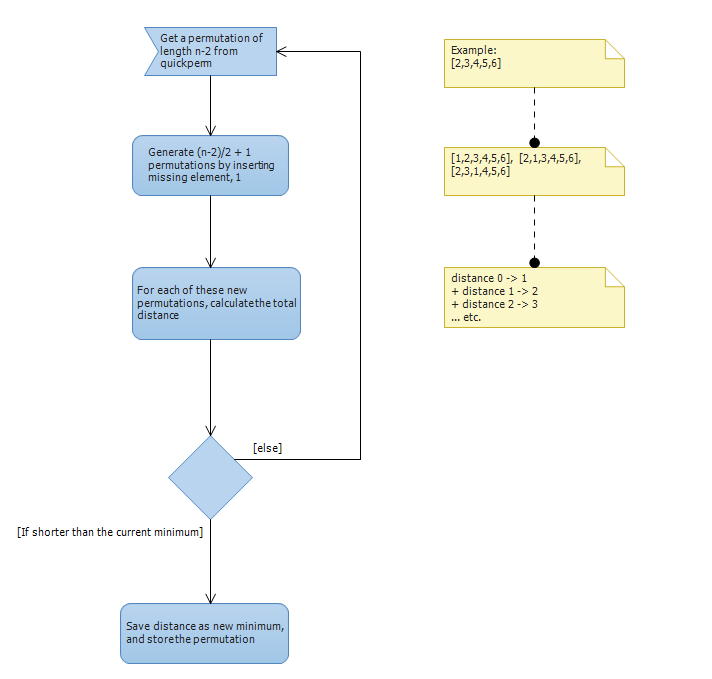
\includegraphics[scale=0.8]{fpga_uml}
\FloatBarrier\noindent
This demonstrates that the majority of reverse permutations are removed from the
generated result. 
\par\bigskip\noindent
Finally, the third improvement considered the parallel capabilities 
of hardware. To speed up the brute force process, 
two variations of the quickperm algorithm run in parallel for large worlds. 
As the size of the world is known, the array being 
permuted, \texttt{a}, and the permutation counting array, \texttt{p}, has a known 
mid-point that can be predetermined. By creating a second copy of the 
\texttt{brute\_force\_tsp} function, and ensuring the two share no data, the calls 
to both occur in parallel. This is verified by checking the analysis tab of 
vivado\_hls:  \\
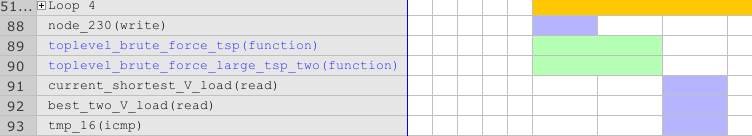
\includegraphics[width=\textwidth]{vivado_hls}
This shows two iterative permutation algorithms occurring in parallel, providing 
a significant speedup in determining the optimal permutation. 

\section{Evaluation and Testing} % 200 words
% Testing strategy. 
For testing the solution, one main method was employed. To
determine the optimal hardware configuration in vivado-hls, a testbench was setup. This
used data printed from the Microblaze for several variations of world sizes and 
ids. This meant that, prior to hardware generation, the hardware was tested and 
verified with data from actual problems. This approach ensured the generated hardware 
behaved as expected, as the testbench and Microblaze code are nearly identical. 
\par\bigskip\noindent
% Performance enhancements
To evaluate the performance enhancements implemented in the final solution,
analysis of the timing for several large worlds was required. This
was achieved by manually timing the solution on several large worlds at each
stage in the optimisation. This is displayed in the following table: 
\begin{table}[!htbp]
\centering
\begin{tabular}{l|lllll}
                  &  &  \textbf{Time taken} & (seconds)          & \\ 
    \textbf{Solution} & World id 1          & World id 2 & World id 3 & World id 4 & Average\\ \hline
    Original Solution    & 33.0             & 36.2       & 36.5   & 34.2 & 35.0 \\ 
    Storing Cost for A*  & 29.9             & 31.4       & 31.2   & 30.3 & 30.7 \\ 
    Using $n!/2$         & 14.0             & 17.5       & 18.0   & 17.1 & 16.7 \\ 
    Parallel Brute force & 7.0              & 8.4        & 8.4    & 7.8  & 7.9 
\end{tabular}
\end{table}
\FloatBarrier\noindent
This shows a 440\% increase in speed over the original implementation,
demonstrating that a high performance solution can be found, capable of handling 
any of the three sizes of problem. 
\bibliographystyle{IEEEtran}
\bibliography{references}
\end{document}
